\documentclass[10pt]{report}
\usepackage{lmodern}
\usepackage[scaled]{helvet}
\renewcommand*\familydefault{\sfdefault} 
\usepackage[T1]{fontenc}
\usepackage{courier}
\usepackage[utf8]{inputenc}
\usepackage{amsmath,amsthm,amsfonts,amssymb,amscd}
\usepackage[a4paper,hmargin=0.8in,bottom=1.3in]{geometry}
\usepackage{lastpage,enumerate,fancyhdr,mathrsfs,xcolor,listings,graphicx,hyperref,enumitem}
\lstset{basicstyle=\footnotesize\ttfamily}
\lstset{
escapeinside={/*!}{!*/}
}
\title{Operating Systems: Shortnotes}
\author{Hardik Rajpal}
\begin{document}
\maketitle
\tableofcontents
\pagebreak
\chapter{Introduction}
\chapter{CPU Virtualization}
\section*{Terms}
\begin{itemize}
\item Process Control Block: A per-process data structure that tracks process meta-data.
\end{itemize}
\chapter{Memory Virtualization}
\section*{Terms}
\begin{enumerate}
    \item Address Space: The running program's view of the memory available to it. Every program only sees the memory available to it, which is split between the code, (static) data, heap and stack.
    \item Sparse Address Space: An address space where most of the
    memory between heap and stack is unused.
    \item Memory Management Unit: The hardware responsible for V2P translation.
    \item Protection Bits: Bits in VA that represent the process'
    access permission for the PA to which it points, including read/write/execute permissions. 
    \item Fragmentation: Wastage of physical memory space.
    \begin{itemize}
        \item Internal: Wastage within a contiguous block of physical memory allocated to a process. An example is the unused space between heap and stack in a simple base-bounds V2P map.
        \item External: Wastage outside of contiguous blocks that have been allocated. This is because of the gaps of available physical memory being too small to fit any new contiguous segments. 
    \end{itemize}
    \item Page: Unit of address space.
    \item Page Frame: Unit of physical address space to which a page can be mapped. Same unit, but \textbf{pages} exist in the
    virtual address space whereas \textbf{page frames} exist
    in the physical address space.
\end{enumerate}
\section{Address Space}
The program is actually loaded into random physical addresses, but due to the address space
abstraction, the program sees the memory available to it as a contiguous chunk, starting at 0.
Every address the program sees is virtual and the OS (with some translation mechanism
of the VA to PA) uses the PA whenever the program references the VA.
\section{Address Translation}
All address translation is hardware-based for efficiency.
Each memory access (load/store) is intercepted by the hardware
and the VA is translated to a PA. The OS helps setup the
hardware for the right translation (per process), and manages memory.
\subsection{Dynamic Relocation a.k.a. (Base, Bound)}
\begin{itemize}
\item Two registers for this in the CPU: base and bound.
\item Translation:
\begin{lstlisting}
V2P(VA v){
    if(v > bound || v < 0){
        throw "Out of Bounds";
    }
    return (base + v);
}
\end{lstlisting}
\item Values of base and bounds for each process are stored in its
PCB.
\item Base and bound registers are privileged: if access is attempted
from user mode, the OS terminates the access-requesting process.
\end{itemize}
\subsection{Segmentation}
\begin{itemize}
\item Generalized base and bounds for each logical segment
of each process: code, heap and stack.
\item Maintain base and size for each segment:
\begin{center}
    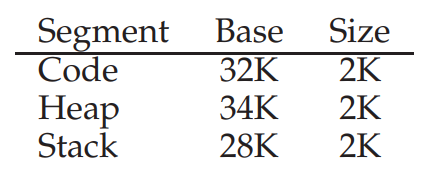
\includegraphics[width=5cm]{res/segmentation.png}
\end{center}

\item Use VA[0:2] to represent the segment type.
\item Better handles \textbf{sparse address spaces}, where
the program often has very little heap and stack data and
thus a lot of the in-between space in a contiguous allocation is 
wasted.
\item Translation is more involved:
\begin{lstlisting}
V2P(VA v){
    segment = v[0:2];//or bit operations.
    offset = v[2:];//or bit operations.
    if(offset < 0 || offset > segdata[segment]["bound"]){
        throw "Out of Bounds"
    }
    else{
        return segdata[segment]["base"] + offset;
    }
}
\end{lstlisting}
\item OS responsibilities:
\begin{itemize}
    \item On each context switch the \textbf{segmentation table} for the process is replaced by the incoming process' table.
    \item On a receiving new process (and its accompanying address 
    space), the OS has to find space in the physical memory for its 
    segments. If the segments are of varying sizes (bounds) this is more involved.
    \item Variable size segments lead to external fragmentation.
    \item A solution to external fragmentation is periodic compaction:
    \begin{enumerate}
        \item Stop running processes.
        \item Copy their data to a contiguous chunk of memory.
        \item Update their segment register values.
    \end{enumerate}
    This creates available contiguous chunks of physical memory but 
    compaction is expensive (copying segments is memory-intensive)
    and would take up a fair amount of CPU time.
    \item Alternative approaches involve using a free-list 
    management algorithm like:
    \begin{itemize}
        \item best-fit
        \item worst-fit
        \item first-fit
        \item buddy algorithm
    \end{itemize} 
    \item External fragmentation will always exist in this scheme,
    however. The algorithms above simply aim to minimize it. The real solution is to disallow variable sized segments.
\end{itemize}
\item Some systems merge code and heap segments to use only one bit
to represent segment.
\item There are \textbf{implicit} approaches to identify the segment too, where the program infers the segment by identifying how the 
VA was conceived:
\begin{itemize}
    \item from a PC $\implies$ use code segment.
    \item from ebp $\implies$ use stack segment.
    \item else, use heap segment.
\end{itemize}
\item We also need an additional bit to identify the direction of growth of the segment, if this varies across the segments. The translation function is modified to take this into account.
\end{itemize}
\subsubsection{Sharing Segments}
\begin{itemize}
\item With some VA bits used to represent permissions that a process
has for the segment \textbf{protection bits}, we can factor include segments with varying
permissions.
\item Translation function is appropriately modified to 
raise an exception whenever a process attempts to violate
permissions for a PA.
\item Read-only code can be shared across multiple processes, without
the worry of harming isolation.
\end{itemize}
\subsubsection{Fine-grained Vs. Coarse-grained}
\begin{itemize}
\item Segments of code, heap and stack are relatively large (coarse-grained segmentation).
\item Fine-grained segmentation further splits up each
of these logical segments and identifies each segment using
a \textbf{segment table}. This allows for better memory
management by the OS (by moving unused segments to disk).
\end{itemize}
\subsection{Paging}
\begin{itemize}
\item Split the address space (abstraction visible to the process) 
into fixed-size units called pages. The corresponding contiguous units in the physical address space are called page frames.
\item To record each page's mapping for each process, the OS
maintains a \textbf{page table} per process.
\item Translation: (neglecting bits other than VPN and offset)
\begin{center}
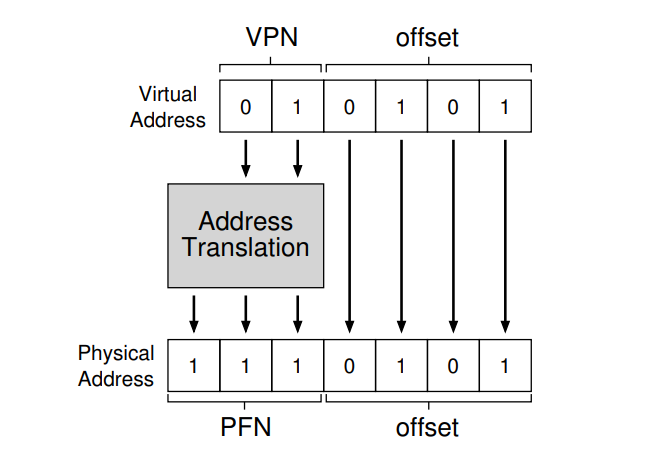
\includegraphics[width=5cm]{res/paging.png}
\end{center}
\end{itemize}

\subsubsection{Inside The Page Table}
\begin{itemize}
\item The OS stores the page table in memory, in units of
\textbf{page table entries} (PTEs).
\item Each PTE has a physical address to which it maps and a collection of metadata bits.
\item The PTEs are stored in a (nested) array-like structure, such
that a VPNs can be used as indices into the structure, pointing
at the PTE that contains their corresponding PFN.
\item The metadata bits:
\begin{enumerate}
    \item Valid bit:indicates whether PTE is valid.
    \begin{itemize}
        \item When a program starts running, all the (virtual) space 
        between the heap and stack is unused and hence unmapped. 
        Hence entries at pagetable [VA] for those addresses are 
        invalid.
        \item If a program tries to access invalid memory, a trap is
        generated and the program is likely terminated.
        \item The valid bit is crucial for supporting \textbf{sparse address spaces}.
        \item Invalid PTEs don't have any physical memory mapped to 
        them, this lets us use only the physical memory we need.
    \end{itemize}
     \item Protection bits: indicate whether the page can be
     read from, written to or executed from. Invalid accesses
     generate a trap to the OS.
     \item Present bit: indicates whether page is present in memory
     (or has been swapped out to disk).
     \item Dirty bit: indicates whether the page has been modified 
     since being loaded into memory.
     \item Reference (a.k.a. accessed) bit: used to track if the
     page has been accessed since the bit was last reset. This 
     information helps in page replacement, to keep popular pages
     around.
     \item User/Supervisor bit: indicates if processes can access
     the page in user mode.
     \item Hardware caching bits: help determine how hardware caching works for the page. 
\end{enumerate}
\end{itemize}
\subsubsection{Advantages of paging}
\begin{itemize}
    \item Flexibility is an important advantage of paging: it works 
    regardless of how the process uses the address space, how the heap
    and stack grow or how they are used.
    \item Simplicity: when new pages are requested, the OS simply
    traverses a free list and returns the first pages that it finds.
\end{itemize}
\section{Free Space Management}
\chapter{Concurrency}
\chapter{Misc.}
\chapter{References}
\begin{enumerate}
\item OSTEP
\end{enumerate}
\end{document}